\documentclass[12pt]{article}
\usepackage[margin=0.75in]{geometry}  % Ajustar márgenes
\usepackage{hyperref}
\usepackage{graphicx}
%\usepackage[margin=1.0in]{geometry}   % sets all margins to 1in, can be changed
%\usepackage{moreverb}                 % for verbatimtabinput -- LaTeX environment
\usepackage{rotating}
\usepackage{url}     
\usepackage{hyperref}
\usepackage{multirow}
\usepackage{amssymb}                  % for many mathematical symbols
\usepackage[pdftex]{lscape}           % for landscaped tables
\usepackage{longtable}
\usepackage[dvipsnames]{xcolor}
\usepackage[spanish]{babel}
\usepackage[utf8]{inputenc}


\newtheorem{Def}{Definici\'on}[section]
\newtheorem{Ejem}{Ejemplo}[section]
\newtheorem{Teo}{Teorema}[section]
\newtheorem{Dem}{Demostraci\'on}[section]
\newtheorem{Note}{Nota}%[section]
\newtheorem{Sol}{Soluci\'on}[section]
\newtheorem{Prop}{Proposici\'on}[section]
\newtheorem{Coro}{Corolario}[section]
\newtheorem{Quest}{Pregunta}[section]

\title{Gu\'ia de estudio en Machine Learning y  Deep Learning}
\author{Carlos E Mart\'inez-Rodr\'iguez}
\date{14  de noviembre de 2023}  % Eliminar la fecha automática

\begin{document}

\maketitle
\tableofcontents
\newpage

%==__== ==__== ==__== ==__== ==__== ==__== ==__== 
\section{An\'alisis de Componentes Principales}
%==__== ==__== ==__== ==__== ==__== ==__== ==__== 

%----------------------------------------------------------------
\subsection{Introduction to Principal Components Analysis - Kristin L.  Sainani}
%----------------------------------------------------------------
Principal components analysis (PCA) is a powerful statistical tool that can help researchers analyze datasets with many highly related predictors. PCA is a data reduction technique -that is, it reduces a larger set of predictor variables to a smaller set with minimal loss of information. PCA may be applied before running regression analyses or for exploratory purposes to help researchers understand relationships among their variables or discover patterns in their data.  Besides compressing the data, PCA analysis also reveals clusters of variables that are highly related, which can give investigators a deeper understanding of their data

\begin{Note}
To illustrate the value of PCA, I will apply the technique to some data pertaining to 91 female adolescent runners. These data come from a larger real dataset [1] but have been modified for use in classroom examples, and thus the results presented here are only for teaching purposes. The researchers measured a large number of potential predictors of bone density and stress fractures, including variables relating to body size and composition, training, per- formance, menstrual function, diet, and eating behaviors. An examination of the correlation coefficients between these 11 variables shows that many are highly related, even across different groups of variables. The application of PCA to these data before performing regression analyses has several benefits. The researchers have collected multiple measurements that reflect the same construct—for example, running performance or menstrual function. If they enter all of these variables into a regression model, they increase the risks of overfitting and type I errors (chance findings). However, if they ignore or discard variables, they lose valuable infor- mation. PCA analysis instead compresses the 11 original variables into a smaller subset of composite variables (called principal components) that capture most of the information in the original data. These new variables may then be used for further analyses. They have the added benefit of being uncorrelated with one another, which makes them easier to interpret and analyze. Before performing PCA analysis on the example data, I first imputed missing values, because observations that have any missing data will otherwise be omitted. I also converted the variables into standard deviation units (Z scores), because all the variables need to have the same units before PCA is applied.
\end{Note}

\subsection{Principal component analysis - 
Herve  Abdi  and Lynne J. Williams}


PCA analyzes a data table representing observations described by several dependent vari- ables, which are, in general, inter-correlated. Its goal is to extract the important information from the data table and to express this information as a set of new orthogonal variables called principal components. PCA also represents the pattern of similarity of the observations and the variables by displaying them as points in maps

\subsection{Approximate Statistical Test for comparing Supervised Classification Learning Algortihms - Dietterich Thomas}

El objetivo  de esta investigaci\'on es encontrar el mejor clasificador o el mejor algoritmo de aprendizaje para ser aplicado en ese dominio. Un objetivo principal en ML es encontrar algoritmos que trabajen bien en un amplio rango de aplicaciones.

\begin{Note}
Un clasificador es una funci\'on que dada un ejemplo de entrada,  a ese ejemplo se le asigne una de las $K$ clases.
\end{Note}


\begin{Note}
Un algoritmo de aprendizaje es una funci\'on  que dado un conjunto de ejemplos y sus clases, construya un clasificador.
\end{Note}

\begin{Note}
En un principio, el objetivo es encontrar el mejor clasificador y estimar su precisi\'on en futuros ejemplos.  En algunas aplicaciones se seleccionar\'a el mejor algoritmo de aprendizaje m\'as que el mejor clasificador.
\end{Note}

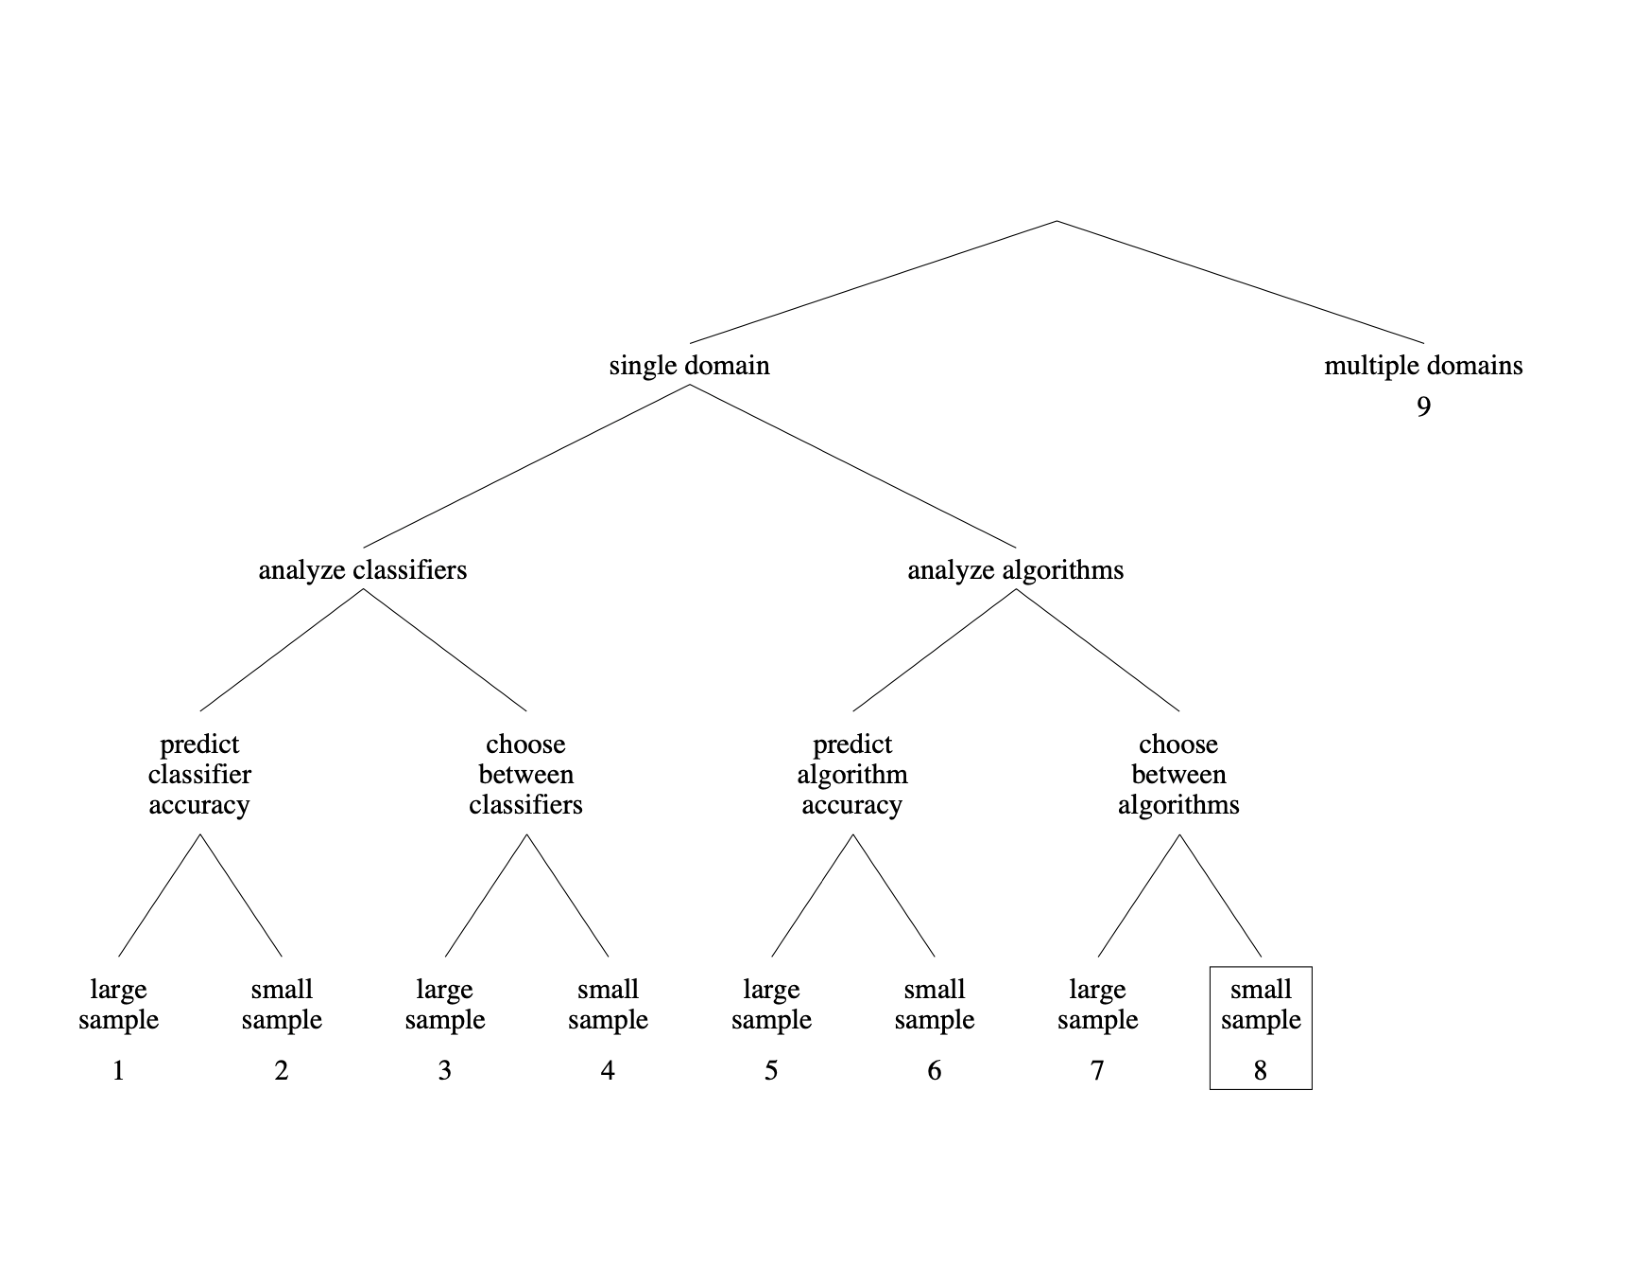
\includegraphics[scale=.5]{TaxonomicalQuestion.pdf} 

El siguiente nivel distingue entre estimar la precisi\'on y elegir clasificadores o algoritmos. El nivel m\'as bajo est\'a relacionado con la cantidad de datos disponibles, si se tiene una gran cantidad de datos, entonces se pueden fijar un conjunto de ellos para ser considerados como datos de prueba para evaluar los clasificadores. En muchos de los casos, la cantidad de datos es limitada y se requeire utilizar todos como datos de entrada a los algoritmos de aprendizaje, esto quiere decir que se requiere utilizar algunas t\'ecnicas de remuestreo para realizar an\'alisis estad\'isticos.

\begin{Note}\textbf{Nueve Preguntas}\\
Se supone que todos los puntos de datos se obtienen de manrea independiente de una distribuci\'on de probabilidad fija definida por el problema en particular.
\begin{Quest}
Sup\'ongase que se tiene una muestra de datos grande y un clasificador $C$. El clasificador pudo haber sido construido utilizando parte de los datos, pero a\'un existen datos para conformar un conjunto de datos de prueba. Por tanto se puede medir la precisi\'on de $C$ en el conjunto de datos de prueba y construir un intervalo de confianza binomial. El clasificador pudo haber sido generado por cualquier m\'etodo y no necesariamente por un algoritmo de aprendizaje.
\end{Quest}

\begin{Quest}
Dado un conjunto de datos peque\~no $S$, sup\'ongase que se aplica un algoritmo de aprendizaje $A$ a $S$ para construir un clasificador $C_{A}$, qu\'e tan preciso es el clasificador $C_A$ para nuevos ejemplos. Dado que no se tienen conjuntos de datos separados no es posible responder la pregunta directamente. Es posible predecir la precisi\'on del algoritmo $A$ cuando se entrena en conjuntos de datos seleccionados aleatoriamente de aproximadamente el mismo tama\~no que $S$. Si esto es posible entonces se puede predecir la precisi\'on de $C_A$ que fue obtenido  despues de ser entrenado en $S$. 

\end{Quest}


\begin{Quest}
Dados dos clasificadores $C_A$ y $C_B$ y suficientes datos para tener un conjunto de datos de prueba, determinar cual clasificador ser\'a m\'as preciso en nuevos ejemplos de prueba.  Esto se puede responder midiendo la precisi\'on de cada clasificador en los datos de prueba y aplicando la prueba de McNemar.

\end{Quest}


\begin{Quest}


\end{Quest}


\begin{Quest}


\end{Quest}


\begin{Quest}


\end{Quest}


\begin{Quest}


\end{Quest}


\begin{Quest}


\end{Quest}


\begin{Quest}


\end{Quest}

\end{Note}



\newpage


\section{Guia de estudio de Machine Learning}

\begin{itemize}
    \item Algoritmos de aprendizaje supervisado:
        \begin{itemize}
            \item Regresión lineal y logística
            \item Máquinas de soporte vectorial (SVM)
            \item Árboles de decisión y bosques aleatorios
            \item Redes neuronales
        \end{itemize}
    \item Aprendizaje no supervisado:
        \begin{itemize}
            \item K-Means y clustering jerárquico
            \item Análisis de componentes principales (PCA)
            \item Algoritmos de asociación
            \item Mapas autoorganizados (SOM)
        \end{itemize}
    \item Evaluación de modelos y métricas:
        \begin{itemize}
            \item Precisión, sensibilidad, especificidad
            \item Curvas ROC y área bajo la curva (AUC-ROC)
            \item Matriz de confusión
            \item Validación cruzada
        \end{itemize}
    \item Preprocesamiento de datos:
        \begin{itemize}
            \item Normalización y estandarización
            \item Manejo de datos faltantes
            \item Ingeniería de características
            \item Selección de características
        \end{itemize}
    \item Optimización de modelos:
        \begin{itemize}
            \item Hiperparámetros y búsqueda en cuadrícula
            \item Optimización bayesiana
            \item Regularización
            \item Redes neuronales convolucionales (CNN) y recurrentes (RNN)
        \end{itemize}
    \item Aprendizaje por refuerzo:
        \begin{itemize}
            \item Q-Learning
            \item Algoritmos de políticas
            \item Exploración y explotación
            \item Funciones de valor
        \end{itemize}
    \item Ética en el machine learning:
        \begin{itemize}
            \item Sesgo y equidad
            \item Transparencia y explicabilidad
            \item Privacidad y seguridad
            \item Responsabilidad en el despliegue de modelos
        \end{itemize}
\end{itemize}


\subsection{SVM}

\begin{enumerate}
    \item \textbf{Hiperplano:}
        En un espacio de características $n$-dimensional, un hiperplano es un subespacio de dimensión $n-1$. Para un problema de clasificación binaria, un hiperplano divide el espacio en dos regiones, asignando puntos a una clase u otra.

    \item \textbf{Margen:}
        El margen es la distancia perpendicular desde el hiperplano a los puntos más cercanos de cada clase. SVM busca el hiperplano que maximiza este margen, lo que se traduce en una mayor robustez y generalización del modelo.

    \item \textbf{Vectores de Soporte:}
        Estos son los puntos de datos más cercanos al hiperplano y tienen un papel crucial en la definición del margen. Cambiar estos vectores de soporte afecta directamente al modelo, y son los únicos puntos que importan para la determinación del hiperplano.

    \item \textbf{Función de Decisión:}
        La función de decisión de SVM es el hiperplano que se utiliza para clasificar nuevos puntos de datos. Dada una entrada, la función de decisión evalúa de qué lado del hiperplano cae el punto y asigna la etiqueta correspondiente.

    \item \textbf{Kernel Trick:}
        SVM puede manejar eficientemente datos no lineales mediante el uso de funciones de kernel. Estas funciones transforman el espacio de características original en uno de mayor dimensión, permitiendo así que los datos sean separados de manera no lineal en el espacio transformado.

    \item \textbf{Parámetros de SVM:}
        \begin{itemize}
            \item \textbf{C (Parámetro de Regularización):} Controla el equilibrio entre tener un margen más amplio y clasificar correctamente los puntos de entrenamiento.
            \item \textbf{Kernel:} Define la función de kernel utilizada (lineal, polinómica, radial, etc.).
            \item \textbf{Gamma (para kernels no lineales):} Controla el alcance de influencia de un solo punto de datos en la decisión.
        \end{itemize}

    \item \textbf{Proceso de Entrenamiento:}
        Dado un conjunto de datos de entrenamiento etiquetado, SVM busca el hiperplano óptimo que maximiza el margen entre las clases. Esto se realiza a través de técnicas de optimización cuadrática.

    \item \textbf{SVM para Regresión:}
        Además de la clasificación, SVM se puede utilizar para problemas de regresión. En este caso, el objetivo es ajustar un hiperplano de modo que contenga la mayor cantidad posible de puntos dentro de un margen predefinido.

    \item \textbf{Ventajas y Desventajas:}
        \begin{itemize}
            \item \textbf{Ventajas:} Efectivo en espacios de alta dimensión, eficaz en conjuntos de datos pequeños y versátil gracias al kernel trick.
            \item \textbf{Desventajas:} Sensible a la escala de las características, puede ser computacionalmente costoso para grandes conjuntos de datos y requiere la elección cuidadosa de parámetros.
        \end{itemize}

    \item \textbf{Aplicaciones:}
        SVM se utiliza en una variedad de campos, como reconocimiento de escritura, clasificación de imágenes, diagnóstico médico, entre otros.

\end{enumerate}


\subsubsection{Elementos Matemáticos de las SVM}

\begin{enumerate}
    \item \textbf{Hiperplano:}
        Un hiperplano se define como \(w \cdot x - b = 0\), donde \(w\) es el vector de pesos, \(x\) es el vector de entrada, y \(b\) es el sesgo.

    \item \textbf{Margen:}
        El margen \(M\) entre un hiperplano y un punto \(x_i\) se define como \(M = \frac{1}{\|w\|} |w \cdot x_i - b|\).

    \item \textbf{Vectores de Soporte:}
        Los vectores de soporte son los puntos \(x_i\) que cumplen la condición \(|w \cdot x_i - b| = 1/\|w\|\).

    \item \textbf{Función de Decisión:}
        La función de decisión es \(f(x) = w \cdot x - b\). Si \(f(x) > 0\), el punto \(x\) se clasifica como clase 1; si \(f(x) < 0\), se clasifica como clase -1.

    \item \textbf{Kernel Trick:}
        La función de kernel \(K(x, x')\) representa el producto escalar en un espacio de características de mayor dimensión. Ejemplos comunes incluyen el kernel lineal (\(K(x, x') = x \cdot x'\)), kernel polinómico (\(K(x, x') = (x \cdot x' + 1)^d\)), y kernel radial (\(K(x, x') = \exp(-\gamma \|x - x'\|^2)\)).

    \item \textbf{Parámetros de SVM:}
        \begin{itemize}
            \item \(C\) (Parámetro de Regularización): Se introduce en la función de pérdida para controlar el equilibrio entre tener un margen más amplio y clasificar correctamente los puntos de entrenamiento.
            \item \(w\) (Vector de Pesos): Aprende durante el entrenamiento y define la orientación del hiperplano.
            \item \(b\) (Sesgo): Parámetro de ajuste del hiperplano.
            \item \(\gamma\) (para kernels no lineales): Controla el alcance de influencia de un solo punto de datos en la decisión.
        \end{itemize}

    \item \textbf{Proceso de Entrenamiento:}
        El proceso de entrenamiento implica la minimización de la función de pérdida, que incluye el término de regularización \(C\|w\|^2\) y la función de pérdida hinge.

    \item \textbf{SVM para Regresión:}
        Para regresión, el objetivo es ajustar un hiperplano de modo que \(|w \cdot x_i - b| \leq \epsilon\) para puntos de entrenamiento \(x_i\).

    \item \textbf{Ventajas y Desventajas:}
        \begin{itemize}
            \item Ventajas: Efectivo en espacios de alta dimensión, eficaz en conjuntos de datos pequeños y versátil gracias al kernel trick.
            \item Desventajas: Sensible a la escala de las características, puede ser computacionalmente costoso para grandes conjuntos de datos y requiere la elección cuidadosa de parámetros.
        \end{itemize}

    \item \textbf{Aplicaciones:}
        SVM se aplica en una variedad de problemas, como reconocimiento de escritura, clasificación de imágenes y diagnóstico médico.
\end{enumerate}


\subsection{Árboles de Decisión}

\begin{enumerate}
    \item \textbf{Definición:}
        Un árbol de decisión es una estructura jerárquica en forma de árbol que se utiliza para representar decisiones y sus posibles consecuencias. Cada nodo interno del árbol representa una prueba en una característica, cada rama representa un resultado posible de la prueba, y cada hoja representa un resultado final o una decisión.

    \item \textbf{Proceso de Construcción:}
        El árbol se construye de manera recursiva. En cada paso, se elige la mejor característica para dividir el conjunto de datos en función de algún criterio, como la ganancia de información o la impureza de Gini. Este proceso se repite hasta que se alcanza algún criterio de parada, como la profundidad máxima del árbol o un número mínimo de puntos en una hoja.

    \item \textbf{Criterios de División:}
        Los criterios comunes para la división incluyen:
        \begin{itemize}
            \item \textbf{Ganancia de Información:} Mide cuánta información nueva proporciona una característica.
            \item \textbf{Impureza de Gini:} Mide la probabilidad de clasificar incorrectamente un elemento si es etiquetado aleatoriamente.
        \end{itemize}

    \item \textbf{Ventajas y Desventajas:}
        \begin{itemize}
            \item \textbf{Ventajas:} Fácil interpretación, no requiere normalización de datos, manejo natural de características categóricas.
            \item \textbf{Desventajas:} Propenso al sobreajuste, especialmente en conjuntos de datos pequeños y ruidosos.
        \end{itemize}
\end{enumerate}

\subsubsection{Bosques Aleatorios}

\begin{enumerate}
    \item \textbf{Definición:}
        Un bosque aleatorio es una colección de árboles de decisión entrenados en subconjuntos aleatorios del conjunto de datos y utilizando técnicas de agregación para mejorar la precisión y controlar el sobreajuste.

    \item \textbf{Proceso de Construcción:}
        Se crean múltiples árboles de decisión utilizando diferentes subconjuntos del conjunto de datos de entrenamiento y características aleatorias en cada división. Luego, las predicciones de cada árbol se promedian (en regresión) o se votan (en clasificación) para obtener la predicción final del bosque.

    \item \textbf{Técnica de Bagging:}
        La construcción de árboles en subconjuntos aleatorios del conjunto de datos se conoce como bagging (bootstrap aggregating). Esto ayuda a reducir la varianza y evitar el sobreajuste al promediar los errores.

    \item \textbf{Importancia de Características:}
        Los bosques aleatorios proporcionan una medida de la importancia de las características, que indica cuánto contribuye cada característica a la precisión del modelo. Esto es útil para la selección de características.

    \item \textbf{Ventajas y Desventajas:}
        \begin{itemize}
            \item \textbf{Ventajas:} Reducción del sobreajuste en comparación con un solo árbol, manejo automático del sobreajuste, buen rendimiento en conjuntos de datos grandes y complejos.
            \item \textbf{Desventajas:} Menos interpretables que los árboles de decisión individuales.
        \end{itemize}
\end{enumerate}

\subsubsection{Elementos Matemáticos de Árboles de Decisión}

\begin{enumerate}
    \item \textbf{Definición:}
        Un árbol de decisión se representa como una función \(T(x)\) que asigna una instancia \(x\) a una hoja del árbol. Cada nodo interno \(j\) realiza una prueba en una característica \(f_j(x)\), y cada rama representa una condición de prueba. La estructura del árbol se define por las funciones indicadoras \(I(x, j)\) que indican si la instancia \(x\) llega al nodo \(j\).
        
        \[ T(x) = \sum_{j=1}^{J} I(x, j) \cdot C_j \]

        Donde \(J\) es el número de nodos, \(C_j\) es el valor en la hoja correspondiente al nodo \(j\), y \(I(x, j)\) es 1 si la instancia \(x\) llega al nodo \(j\) y 0 de lo contrario.

    \item \textbf{Proceso de Construcción:}
        La construcción del árbol implica seleccionar la mejor característica \(f_j\) y el umbral \(t_j\) en cada nodo \(j\) para maximizar la ganancia de información o reducir la impureza de Gini.
        
        \[ \textrm{Ganancia de Información: } Gain(D, j, t) = H(D) - \frac{N_L}{N} H(D_L) - \frac{N_R}{N} H(D_R) \]

        \[ \textrm{Impureza de Gini: } Gini(D) = 1 - \sum_{k=1}^{K} \left(\frac{|C_k|}{|D|}\right)^2 \]

        Donde \(D\) es el conjunto de datos en el nodo, \(D_L\) y \(D_R\) son los conjuntos de datos en los nodos izquierdo y derecho después de la división, \(N\) es el número total de instancias en \(D\), y \(N_L\) y \(N_R\) son los números de instancias en los nodos izquierdo y derecho.

    \item \textbf{Ventajas y Desventajas:}
        \begin{itemize}
            \item \textbf{Ventajas:} Fácil interpretación, no requiere normalización de datos, manejo natural de características categóricas.
            \item \textbf{Desventajas:} Propenso al sobreajuste, especialmente en conjuntos de datos pequeños y ruidosos.
        \end{itemize}
\end{enumerate}

\subsubsection{Bosques Aleatorios}

\begin{enumerate}
    \item \textbf{Definición:}
        Un bosque aleatorio es una colección de \(B\) árboles de decisión \(T_b(x)\), donde cada árbol se entrena en un subconjunto aleatorio de los datos de entrenamiento. La predicción se obtiene promediando (en regresión) o votando (en clasificación) las predicciones individuales de los árboles.

        \[ \textrm{Predicción del Bosque: } \hat{Y}(x) = \frac{1}{B} \sum_{b=1}^{B} T_b(x) \]

    \item \textbf{Proceso de Construcción:}
        Cada árbol en el bosque se construye utilizando bagging, que consiste en seleccionar aleatoriamente un subconjunto de las instancias de entrenamiento con reemplazo. Además, en cada división de nodo, se selecciona un subconjunto aleatorio de características.

        \[ \textrm{Bagging: } D_b = \{(x_i, y_i)\} \textrm{ con } i \sim \textrm{Uniforme}(1, N) \]

        \[ \textrm{Características Aleatorias: } f_j \textrm{ con } j \sim \textrm{Uniforme}(1, P) \]

    \item \textbf{Importancia de Características:}
        La importancia de la característica \(f_j\) se mide mediante la disminución promedio en la ganancia de impureza o la reducción en el error cuadrático medio cuando se utiliza \(f_j\) para dividir los nodos a lo largo de todos los árboles.

        \[ \textrm{Importancia de } f_j = \frac{1}{B} \sum_{b=1}^{B} \sum_{j \textrm{ en } T_b} \textrm{Importancia de } f_j \textrm{ en } T_b \]

\end{enumerate}








\section{Referencias}
\begin{itemize}
    \item Libros:
        \begin{enumerate}
            \item "The Hundred-Page Machine Learning Book" por Andriy Burkov
            \item "Machine Learning: A Probabilistic Perspective" por Kevin P. Murphy
            \item "Hands-On Machine Learning with Scikit-Learn, Keras, and TensorFlow" por Aurélien Géron
            \item "Pattern Recognition and Machine Learning" por Christopher M. Bishop
            \item "Deep Learning" por Ian Goodfellow, Yoshua Bengio y Aaron Courville
        \end{enumerate}
    \item Cursos:
        \begin{enumerate}
            \item "Machine Learning" por Andrew Ng en Coursera
            \item "Applied Data Science with Python" por la Universidad de Míchigan en Coursera
            \item "Deep Learning Specialization" por Andrew Ng en Coursera
            \item "Machine Learning Crash Course" por Google
            \item "Introduction to Machine Learning" por la Universidad de Columbia en edX
        \end{enumerate}
    \item Sitios web:
        \begin{enumerate}
            \item Kaggle
            \item GitHub
            \item Towards Data Science
            \item Machine Learning Mastery
            \item Google AI
        \end{enumerate}
\end{itemize}


Fuentes:
\begin{enumerate}
    \item Machine Learning citation style [Update October 2023] - Paperpile
    \item ICML2021 Template - Overleaf, Online LaTeX Editor
    \item Machine Learning | Submission guidelines - Springer
    \item Journal of Machine Learning Research
\end{enumerate}

%== == ==  == == == ==  == == == ==  == == == ==  == == == ==  == 
\section{Bioinformatics: New revision}
%== == ==  == == == ==  == == == ==  == == == ==  == == == ==  == 

%-- -- -- -- -- -- -- -- -- -- -- -- -- -- -- -- -- -- -- -- -- -- -- -- -- -- -- -- -- -- 
\subsection{A bayesian framework for combining gene predictions - Pavlovic}
%-- -- -- -- -- -- -- -- -- -- -- -- -- -- -- -- -- -- -- -- -- -- -- -- -- -- -- -- -- -- 

Biology and biotechnology are undergoing a techonolgical revolution which is transforming research into an information-rich enterprise.  A typical bacterial genome sequence is comprised of several million bases of DNA and contains several thousand genes. The human genome is approximately 3 billion bases long and it contains approximately 30,000 putative genes identified thus far.



%== == ==  == == == ==  == == == ==  == == == ==  == == == ==  == 
\section{Random Forest: Explanation in Mathematical Terms}

Random Forest is a supervised learning algorithm used for both classification and regression problems. The main idea behind Random Forest is to build multiple decision trees during training and combine their results to obtain a more robust and accurate prediction.

Let's assume we have a training dataset \(D = \{(x_1, y_1), (x_2, y_2), \ldots, (x_n, y_n)\}\), where \(x_i\) represents the features and \(y_i\) is the target variable.

\begin{enumerate}
    \item \textbf{Construction of Decision Trees:}
        \begin{itemize}
            \item For each tree, a random subset of features is selected (randomly sample features), and a random subset of training data is chosen (randomly sample observations with replacement).
            \item A decision tree is constructed using the subset of data and features.
            \item The decision tree is represented as \(h_i(x;\theta_i)\), where \(i\) denotes the tree index, \(x\) is the input feature vector, and \(\theta_i\) represents the parameters of the tree.
            \item At each node \(t\) of the tree, a feature \(j_t\) is selected from the random subset, and the split is determined based on minimizing impurity:
            \[
            \theta_{i,t} = \arg\min_{j_t, s_t} \left[\textrm{Impurity}(D_t) - p_{\textrm{left}}\textrm{Impurity}(D_{\textrm{left}}) - p_{\textrm{right}}\textrm{Impurity}(D_{\textrm{right}})\right]
            \]
            where \(D_t\) is the dataset at node \(t\), \(D_{\textrm{left}}\) and \(D_{\textrm{right}}\) are the datasets in the left and right child nodes, \(p_{\textrm{left}}\) and \(p_{\textrm{right}}\) are the proportions of data in the left and right child nodes, and \(\textrm{Impurity}(\cdot)\) is a measure of impurity, such as Gini index for classification or mean squared error for regression.
        \end{itemize}
    
    \item \textbf{Voting or Averaging:}
        \begin{itemize}
            \item For classification problems, the final prediction is obtained by majority voting among the trees:
            \[
            H(x) = \textrm{mode}\{h_1(x;\theta_1), h_2(x;\theta_2), \ldots, h_n(x;\theta_n)\}
            \]
            \item For regression problems, the final prediction is the average of predictions from all trees:
            \[
            H(x) = \frac{1}{n}\sum_{i=1}^{n}h_i(x;\theta_i)
            \]
        \end{itemize}
    
    \item \textbf{Variance Reduction:}
        \begin{itemize}
            \item By building decision trees in a random manner, the variance of the model is reduced, leading to a more robust and generalizable model.
        \end{itemize}
\end{enumerate}

The final prediction is obtained by combining the predictions of all trees.

\section{Deep Learning: Overview}

Deep Learning is a subfield of machine learning that focuses on neural networks with multiple layers (deep neural networks). These networks can automatically learn hierarchical representations of data, allowing them to capture intricate patterns and features.

\begin{enumerate}
    \item \textbf{Neural Network Representation:}
        \begin{itemize}
            \item A neural network consists of layers of interconnected nodes (neurons) organized into an input layer, one or more hidden layers, and an output layer.
            \item The input layer represents the features of the data, and each neuron in the layer processes a specific feature.
            \item Hidden layers perform nonlinear transformations on the input data, learning hierarchical representations.
            \item The output layer produces the final prediction based on the learned representations.
        \end{itemize}
    
    \item \textbf{Training a Neural Network:}
        \begin{itemize}
            \item During training, the network's parameters (weights and biases) are adjusted to minimize the difference between predicted and actual outputs.
            \item This optimization is typically done using backpropagation and gradient descent.
        \end{itemize}
    
    \item \textbf{Activation Functions:}
        \begin{itemize}
            \item Activation functions introduce nonlinearity to the neural network, enabling it to learn complex patterns.
            \item Common activation functions include ReLU (Rectified Linear Unit), Sigmoid, and Hyperbolic Tangent (tanh).
        \end{itemize}
    
    \item \textbf{Forward Pass:}
        \begin{itemize}
            \item The forward pass of a neural network involves computing the output of the network for a given input.
            \item Given an input vector \(x\), the output \(y\) is computed by passing \(x\) through the network's layers using learned weights and biases.
            \item The output of each layer is computed as:
            \[
            a^{(l)} = W^{(l)}a^{(l-1)} + b^{(l)}
            \]
            where \(W^{(l)}\) is the weight matrix, \(a^{(l)}\) is the activation of layer \(l\), \(a^{(l-1)}\) is the activation of the previous layer, and \(b^{(l)}\) is the bias vector.
            \item The activation function is then applied to \(a^{(l)}\) to introduce nonlinearity.
        \end{itemize}
    
    \item \textbf{Loss Function:}
        \begin{itemize}
            \item The loss function measures the difference between the predicted output and the true output.
            \item Common loss functions include mean squared error for regression and cross-entropy for classification.
            \item The goal during training is to minimize the loss by adjusting the network's parameters.
        \end{itemize}
    
    \item \textbf{Backpropagation:}
        \begin{itemize}
            \item Backpropagation is a training algorithm that computes the gradient of the loss with respect to the network's parameters.
            \item The gradient is used to update the parameters in the direction that reduces the loss.
            \item It involves computing the gradient of the loss with respect to the output of each layer and using the chain rule to propagate these gradients backward through the network.
        \end{itemize}
\end{enumerate}

\section{Example of Implementation in R:}

\subsection{Install and Load the Keras Library:}
\begin{verbatim}
install.packages("keras")
library(keras)
\end{verbatim}

\subsection{Build a Simple Neural Network:}
\begin{verbatim}
model <- keras_model_sequential() %>%
  layer_dense(units = 128, activation = 'relu', input_shape = c(10)) %>%
  layer_dense(units = 1, activation = 'sigmoid')

summary(model)
\end{verbatim}

\subsection{Compile and Train the Neural Network:}
\begin{verbatim}
model %>% compile(
  optimizer = 'adam',
  loss = 'binary_crossentropy',
  metrics = c('accuracy')
)

# Assuming you have training data X_train and labels y_train
history <- model %>% fit(
  X_train, y_train,
  epochs = 10, batch_size = 32,
  validation_split = 0.2
)
\end{verbatim}

\subsection{Evaluate the Model:}
\begin{verbatim}
# Assuming you have test data X_test and labels y_test
evaluate_result <- model %>% evaluate(X_test, y_test)
print(evaluate_result)
\end{verbatim}


\section{Impurity Measures in Random Forest}

In the context of Random Forest, impurity measures play a crucial role in the construction of decision trees. The two commonly used impurity measures are the Gini index for classification and the mean squared error for regression.

\subsection{Gini Index for Classification}

The Gini index is a measure of impurity used in classification problems. Given a node in a decision tree that contains data points from different classes, the Gini index quantifies how often a randomly chosen data point would be incorrectly classified.

For a node \(t\) with \(K\) classes and a set of data points \(D_t\), the Gini index (\(Gini(t)\)) is calculated as follows:

\[ Gini(t) = 1 - \sum_{i=1}^{K} p_i^2 \]

where \(p_i\) is the proportion of data points in class \(i\) at node \(t\). A lower Gini index indicates a purer node with predominantly one class.

In the context of Random Forest, the decision tree split is determined by minimizing the weighted sum of Gini indices for the left and right child nodes. The split that results in the lowest overall Gini index is chosen.

\subsection{Mean Squared Error for Regression}

For regression problems, the impurity measure used is the mean squared error (MSE). Unlike classification, where impurity is related to the purity of classes in a node, regression impurity is a measure of the variability of target values within a node.

For a node \(t\) with data points \(D_t\), the MSE (\(MSE(t)\)) is calculated as follows:

\[ MSE(t) = \frac{1}{|D_t|} \sum_{i \in D_t} (y_i - \bar{y}_t)^2 \]

where \(y_i\) is the target value of data point \(i\), \(|D_t|\) is the number of data points in node \(t\), and \(\bar{y}_t\) is the mean target value of all data points in node \(t\).

Similar to the Gini index, in Random Forest, the decision tree split is determined by minimizing the weighted sum of MSE for the left and right child nodes.

These impurity measures guide the construction of individual decision trees within the Random Forest ensemble, contributing to the overall robustness and predictive power of the model.


\section{Construcción del Árbol de Decisión}

\subsection{Teoría:}

Un árbol de decisión es una estructura de datos que representa un conjunto de decisiones y sus posibles consecuencias. En el contexto de Random Forest, la construcción de un árbol de decisión sigue el principio de "aprendizaje supervisado", donde el algoritmo aprende patrones a partir de un conjunto de datos etiquetado.

La construcción del árbol se realiza a través de divisiones recursivas basadas en características del conjunto de datos. Cada nodo del árbol representa una pregunta sobre una característica, y las ramas que surgen de ese nodo son las respuestas a esa pregunta. El proceso continúa hasta que se alcanza un criterio de parada, como la profundidad máxima del árbol o el número mínimo de muestras en un nodo.

\subsection{Elementos Matemáticos:}

1. \textbf{Función de Impureza:}

En cada nodo del árbol, se elige la característica y el umbral que minimizan la impureza en los nodos hijos resultantes. La impureza se mide mediante funciones como el Índice de Gini para clasificación o el Error Cuadrático Medio (MSE) para regresión.

Para clasificación:
\[ Gini(t) = 1 - \sum_{i=1}^{K} p_i^2 \]

Donde \( p_i \) es la proporción de ejemplos de la clase \( i \) en el nodo \( t \).

Para regresión:
\[ MSE(t) = \frac{1}{|D_t|} \sum_{i \in D_t} (y_i - \bar{y}_t)^2 \]

Donde \( D_t \) es el conjunto de datos en el nodo \( t \), \( y_i \) es la etiqueta del ejemplo \( i \), y \( \bar{y}_t \) es la media de las etiquetas en el nodo \( t \).

2. \textbf{Criterio de División:}

La elección de la mejor característica y umbral se basa en la reducción de la impureza. Se busca el par \((j, s)\) que minimiza la expresión:
\[ \theta_{i,t} = \arg\min_{j, s} \left[ \textrm{Impureza}(D_t) - p_{\textrm{left}}\textrm{Impureza}(D_{\textrm{left}}) - p_{\textrm{right}}\textrm{Impureza}(D_{\textrm{right}}) \right] \]

Donde \(D_t\) es el conjunto de datos en el nodo \(t\), \(D_{\textrm{left}}\) y \(D_{\textrm{right}}\) son los conjuntos de datos en los nodos izquierdo y derecho después de la división, y \(p_{\textrm{left}}\) y \(p_{\textrm{right}}\) son las proporciones de datos en esos nodos.

3. \textbf{Criterios de Parada:}

Para evitar sobreajuste, se utilizan criterios de parada, como la profundidad máxima del árbol o el número mínimo de muestras requeridas para realizar una división.

La construcción de cada árbol en Random Forest implica este proceso iterativo y se repite para cada árbol en el bosque. La diversidad en la construcción de árboles se logra mediante el uso de diferentes subconjuntos aleatorios de características y datos en cada árbol. La combinación de predicciones de estos árboles mejora la generalización del modelo y su capacidad predictiva en nuevos datos.



\section{Reducción de Varianza en Random Forest}

\subsection{Teoría:}

La reducción de la varianza es uno de los objetivos clave en la construcción de árboles de decisión en Random Forest. Esta técnica busca mejorar la generalización del modelo al reducir la sensibilidad a pequeñas variaciones en los datos de entrenamiento.

La varianza se refiere a la variabilidad de las predicciones de un modelo respecto a diferentes conjuntos de datos de entrenamiento. En Random Forest, la reducción de la varianza se logra mediante dos técnicas principales: Bagging y Random Subspace.

\subsubsection{Bagging (Bootstrap Aggregating):}

Bagging es una técnica que consiste en entrenar múltiples modelos en diferentes subconjuntos de datos generados mediante muestreo con reemplazo (bootstrap). Cada árbol de decisión en Random Forest se entrena en un conjunto de datos ligeramente diferente, lo que introduce diversidad en los modelos.

\subsubsection{Random Subspace:}

Random Subspace es otra técnica utilizada para reducir la correlación entre los árboles de decisión. En lugar de usar todas las características para cada árbol, se selecciona un subconjunto aleatorio de características para entrenar cada árbol. Esto ayuda a que cada árbol se especialice en diferentes aspectos de los datos, mejorando la diversidad y reduciendo la correlación entre las predicciones.

\subsection{Elementos Matemáticos:}

La reducción de la varianza no se expresa directamente con fórmulas matemáticas específicas, pero los conceptos clave son fundamentales:

1. **Bagging:**
    - Cada árbol \(T_i\) se entrena en un conjunto de datos \(D_i\) generado por muestreo con reemplazo (bootstrap).
    - La predicción final se obtiene promediando las predicciones de todos los árboles:
        \[ H(x) = \frac{1}{N} \sum_{i=1}^{N} T_i(x) \]

2. **Random Subspace:**
    - Cada árbol \(T_i\) se entrena utilizando un subconjunto aleatorio de características.
    - La predicción final se obtiene promediando las predicciones de todos los árboles:
        \[ H(x) = \frac{1}{N} \sum_{i=1}^{N} T_i(x) \]

Estos enfoques combinados contribuyen a reducir la varianza del modelo, lo que resulta en un modelo más robusto y generalizable.

\section{Votación y Promedio en Random Forest}

\subsection{Teoría:}

La técnica de "Votación" (para problemas de clasificación) o "Promedio" (para problemas de regresión) es crucial en Random Forest para combinar las predicciones de múltiples árboles de decisión y obtener una predicción final más robusta y precisa.

\subsubsection{Para Problemas de Clasificación:}

En problemas de clasificación, el enfoque de votación se utiliza. Cada árbol en el bosque emite una predicción de clase, y la clase final se determina por mayoría de votos.

\subsubsection{Para Problemas de Regresión:}

En problemas de regresión, se utiliza un enfoque de promedio. Cada árbol realiza una predicción numérica, y la predicción final es el promedio de todas las predicciones.

\subsection{Elementos Matemáticos:}

1. \textbf{Votación para Clasificación:}
    - La predicción final para un ejemplo \(x\) se obtiene por mayoría de votos:
        \[ H(x) = \textrm{mode}\{T_1(x), T_2(x), ..., T_N(x)\} \]

2. \textbf{Promedio para Regresión:}
    - La predicción final para un ejemplo \(x\) se obtiene promediando las predicciones de todos los árboles:
        \[ H(x) = \frac{1}{N}\sum_{i=1}^{N} T_i(x) \]

Donde \(T_i(x)\) representa la predicción del árbol \(i\) para el ejemplo \(x\), y \(N\) es el número total de árboles en el bosque.

Estos enfoques de votación y promedio permiten que Random Forest combine la información de múltiples árboles de decisión, mejorando la generalización y la capacidad predictiva del modelo.

\section{Resumen}

Random Forest es un algoritmo de aprendizaje automático que se utiliza para resolver problemas de clasificación y regresión. En lugar de utilizar un único árbol de decisión, Random Forest construye varios árboles de decisión y los combina para obtener una predicción más precisa. Cada árbol de decisión se construye utilizando un subconjunto aleatorio de las características del conjunto de datos original. Al final, las predicciones de cada árbol se promedian para obtener una predicción final.

El algoritmo de Random Forest se basa en dos técnicas: Bagging y Random Subspace. Bagging es una técnica que se utiliza para reducir la varianza de un modelo al entrenar múltiples modelos en diferentes subconjuntos de datos. Random Subspace es una técnica que se utiliza para reducir la correlación entre los modelos al entrenar cada modelo en diferentes subconjuntos de características.

Aquí hay algunos elementos matemáticos que se utilizan en Random Forest:

\begin{itemize}
    \item \textbf{Árbol de decisión:} Un árbol de decisión es una estructura de datos que se utiliza para modelar decisiones y sus posibles consecuencias. Cada nodo en el árbol representa una decisión, y cada rama representa una posible consecuencia de esa decisión. Los árboles de decisión se construyen utilizando un conjunto de reglas que se utilizan para tomar decisiones.
    \item \textbf{Bootstrap:} Bootstrap es una técnica que se utiliza para generar múltiples conjuntos de datos a partir de un conjunto de datos original. Cada conjunto de datos se genera mediante muestreo con reemplazo, lo que significa que cada elemento del conjunto de datos original tiene la misma probabilidad de ser seleccionado en cada conjunto de datos generado.
    \item \textbf{Out-of-Bag Error:} Out-of-Bag Error es una técnica que se utiliza para estimar el error de validación de un modelo sin la necesidad de un conjunto de datos de validación separado. El error se estima utilizando los datos que no se incluyeron en el conjunto de datos de entrenamiento para cada árbol de decisión.
\end{itemize}

\subsection{Ejemplo en R: Random Forest}

Aquí hay un ejemplo de cómo construir un modelo de bosque aleatorio en R:

\begin{verbatim}
# Cargamos el paquete necesario para este ejemplo
library(randomForest)

# Cargamos el conjunto de datos que deseamos utilizar
data(iris)

# Dividimos el conjunto de datos en conjuntos de entrenamiento y prueba
trainIndex <- createDataPartition(iris$Species, p = .8, list = FALSE, times = 1)

# Entrenamos el modelo de bosque aleatorio
rf_model <- randomForest(Species ~ ., data = iris[trainIndex,])

# Realizamos predicciones en el conjunto de prueba
predictions <- predict(rf_model, iris[-trainIndex,])
\end{verbatim}

\subsection{Deep Learning}

Deep Learning es un subcampo del aprendizaje automático que se centra en la creación de redes neuronales artificiales profundas. Estas redes neuronales están diseñadas para imitar el cerebro humano y son capaces de aprender patrones complejos en los datos.

Aquí hay un ejemplo de cómo construir una red neuronal profunda en R utilizando el paquete keras:

\begin{verbatim}
# Cargamos los paquetes necesarios
library(keras)
library(tensorflow)

# Cargamos el conjunto de datos que deseamos utilizar
data(iris)

# Dividimos el conjunto de datos en conjuntos de entrenamiento y prueba
trainIndex <- createDataPartition(iris$Species, p = .8, list = FALSE, times = 1)

# Creamos la red neuronal
model <- keras_model_sequential() %>% 
  layer_dense(units = 4, input_shape = c(4)) %>% 
  layer_activation("relu") %>% 
  layer_dense(units = 3) %>% 
  layer_activation("softmax")

# Compilamos la red neuronal
model %>% compile(loss = "categorical_crossentropy", optimizer = "adam", metrics = "accuracy")

# Entrenamos la red neuronal
history <- model %>% fit(
  x = iris[trainIndex, 1:4],
  y = to_categorical(as.numeric(iris[trainIndex, 5])),
  epochs = 100,
  batch_size = 10,
  validation_split = 0.2
)
\end{verbatim}



% ===_-_===_-_===_-_===_-_===_-_===_-_===
\section{Algoritmos de Aprendizaje Supervisado}
% ===_-_===_-_===_-_===_-_===_-_===_-_===

%__________________________________
\subsection{Regresión Lineal y Logística}
%__________________________________
    % Contenido sobre regresión lineal y logística
\subsubsection{Regresión Lineal}

La regresión lineal es un modelo que busca modelar la relación lineal entre una variable dependiente \(Y\) y una o más variables independientes \(X\). El modelo se define como:

\[
Y = \beta_0 + \beta_1 X + \varepsilon
\]

donde:
\begin{itemize}
    \item \(Y\) es la variable dependiente que queremos predecir.
    \item \(X\) es la variable independiente que utilizamos para la predicción.
    \item \(\beta_0\) es la ordenada al origen, que representa el valor de \(Y\) cuando \(X\) es cero.
    \item \(\beta_1\) es la pendiente de la recta, que indica cuánto cambia \(Y\) por un cambio unitario en \(X\).
    \item \(\varepsilon\) es el término de error que captura la variabilidad no explicada por el modelo.
\end{itemize}

El objetivo es encontrar los valores de \(\beta_0\) y \(\beta_1\) que minimizan la suma de los cuadrados de los errores \(\varepsilon\):

\[
\min_{\beta_0, \beta_1} \sum_{i=1}^{n} (Y_i - (\beta_0 + \beta_1 X_i))^2
\]

Esto se puede hacer utilizando técnicas como el método de mínimos cuadrados.

\subsubsection{Regresión Logística}

La regresión logística es un modelo utilizado para problemas de clasificación binaria. Se emplea la función logística, también conocida como la función sigmoide, para transformar la salida de la regresión lineal en un valor entre 0 y 1, que se interpreta como la probabilidad de pertenecer a la clase positiva. La función sigmoide está definida como:

\[
P(Y=1) = \frac{1}{1 + e^{-(\beta_0 + \beta_1 X)}}
\]

donde:
\begin{itemize}
    \item \(P(Y=1)\) es la probabilidad de pertenecer a la clase positiva.
    \item \(e\) es la base del logaritmo natural.
\end{itemize}

El modelo de regresión logística busca encontrar los valores de \(\beta_0\) y \(\beta_1\) que maximizan la función de verosimilitud. La función de verosimilitud es el producto de las probabilidades condicionales de observar las etiquetas de clase dados los valores de \(X\):

\[
\max_{\beta_0, \beta_1} \mathcal{L}(\beta_0, \beta_1) = \prod_{i=1}^{n} P(Y_i)^{y_i} \cdot (1 - P(Y_i))^{1 - y_i}
\]

donde:
\begin{itemize}
    \item \(\mathcal{L}(\beta_0, \beta_1)\) es la función de verosimilitud.
    \item \(y_i\) es la etiqueta de la clase para la observación \(i\).
\end{itemize}

La regresión logística se ajusta típicamente maximizando la log-verosimilitud para obtener estimaciones de \(\beta_0\) y \(\beta_1\).

\subsubsection{Implementacion}
\begin{verbatim}
# Ejemplo de Regresión Lineal
set.seed(123)
# Crear datos de ejemplo
X <- rnorm(100)
Y <- 2 * X + rnorm(100)

# Ajustar el modelo de regresión lineal
modelo_lineal <- lm(Y ~ X)

# Imprimir resultados
summary(modelo_lineal)

# Graficar el modelo
plot(X, Y, main = "Regresión Lineal", xlab = "X", ylab = "Y")
abline(modelo_lineal, col = "red")

# Ejemplo de Regresión Logística
set.seed(123)
# Crear datos de ejemplo para clasificación binaria
X <- rnorm(100)
probabilidades <- exp(2 * X) / (1 + exp(2 * X))
Y_binario <- rbinom(100, 1, probabilidades)

# Ajustar el modelo de regresión logística
modelo_logistico <- glm(Y_binario ~ X, family = binomial)

# Imprimir resultados
summary(modelo_logistico)

# Graficar el modelo
plot(X, Y_binario, main = "Regresión Logística", 
         xlab = "X", ylab = "Y", col = Y_binario + 1)
curve(predict(modelo_logistico, 
           data.frame(X = x), type = "response"), 
           add = TRUE, col = "red")
\end{verbatim}


%__________________________________
\subsection{Máquinas de Soporte Vectorial (SVM)}
%__________________________________
    % Contenido sobre SVM

\begin{enumerate}
    \item \textbf{Hiperplano:}
        En un espacio de características $n$-dimensional, un hiperplano es un subespacio de dimensión $n-1$. Para un problema de clasificación binaria, un hiperplano divide el espacio en dos regiones, asignando puntos a una clase u otra.

    \item \textbf{Margen:}
        El margen es la distancia perpendicular desde el hiperplano a los puntos más cercanos de cada clase. SVM busca el hiperplano que maximiza este margen, lo que se traduce en una mayor robustez y generalización del modelo.

    \item \textbf{Vectores de Soporte:}
        Estos son los puntos de datos más cercanos al hiperplano y tienen un papel crucial en la definición del margen. Cambiar estos vectores de soporte afecta directamente al modelo, y son los únicos puntos que importan para la determinación del hiperplano.

    \item \textbf{Función de Decisión:}
        La función de decisión de SVM es el hiperplano que se utiliza para clasificar nuevos puntos de datos. Dada una entrada, la función de decisión evalúa de qué lado del hiperplano cae el punto y asigna la etiqueta correspondiente.

    \item \textbf{Kernel Trick:}
        SVM puede manejar eficientemente datos no lineales mediante el uso de funciones de kernel. Estas funciones transforman el espacio de características original en uno de mayor dimensión, permitiendo así que los datos sean separados de manera no lineal en el espacio transformado.

    \item \textbf{Parámetros de SVM:}
        \begin{itemize}
            \item \textbf{C (Parámetro de Regularización):} Controla el equilibrio entre tener un margen más amplio y clasificar correctamente los puntos de entrenamiento.
            \item \textbf{Kernel:} Define la función de kernel utilizada (lineal, polinómica, radial, etc.).
            \item \textbf{Gamma (para kernels no lineales):} Controla el alcance de influencia de un solo punto de datos en la decisión.
        \end{itemize}

    \item \textbf{Proceso de Entrenamiento:}
        Dado un conjunto de datos de entrenamiento etiquetado, SVM busca el hiperplano óptimo que maximiza el margen entre las clases. Esto se realiza a través de técnicas de optimización cuadrática.

    \item \textbf{SVM para Regresión:}
        Además de la clasificación, SVM se puede utilizar para problemas de regresión. En este caso, el objetivo es ajustar un hiperplano de modo que contenga la mayor cantidad posible de puntos dentro de un margen predefinido.

    \item \textbf{Ventajas y Desventajas:}
        \begin{itemize}
            \item \textbf{Ventajas:} Efectivo en espacios de alta dimensión, eficaz en conjuntos de datos pequeños y versátil gracias al kernel trick.
            \item \textbf{Desventajas:} Sensible a la escala de las características, puede ser computacionalmente costoso para grandes conjuntos de datos y requiere la elección cuidadosa de parámetros.
        \end{itemize}

    \item \textbf{Aplicaciones:}
        SVM se utiliza en una variedad de campos, como reconocimiento de escritura, clasificación de imágenes, diagnóstico médico, entre otros.

\end{enumerate}


\subsubsection{Elementos Matemáticos de las SVM}

\begin{enumerate}
    \item \textbf{Hiperplano:}
        Un hiperplano se define como \(w \cdot x - b = 0\), donde \(w\) es el vector de pesos, \(x\) es el vector de entrada, y \(b\) es el sesgo.

    \item \textbf{Margen:}
        El margen \(M\) entre un hiperplano y un punto \(x_i\) se define como \(M = \frac{1}{\|w\|} |w \cdot x_i - b|\).

    \item \textbf{Vectores de Soporte:}
        Los vectores de soporte son los puntos \(x_i\) que cumplen la condición \(|w \cdot x_i - b| = 1/\|w\|\).

    \item \textbf{Función de Decisión:}
        La función de decisión es \(f(x) = w \cdot x - b\). Si \(f(x) > 0\), el punto \(x\) se clasifica como clase 1; si \(f(x) < 0\), se clasifica como clase -1.

    \item \textbf{Kernel Trick:}
        La función de kernel \(K(x, x')\) representa el producto escalar en un espacio de características de mayor dimensión. Ejemplos comunes incluyen el kernel lineal (\(K(x, x') = x \cdot x'\)), kernel polinómico (\(K(x, x') = (x \cdot x' + 1)^d\)), y kernel radial (\(K(x, x') = \exp(-\gamma \|x - x'\|^2)\)).

    \item \textbf{Parámetros de SVM:}
        \begin{itemize}
            \item \(C\) (Parámetro de Regularización): Se introduce en la función de pérdida para controlar el equilibrio entre tener un margen más amplio y clasificar correctamente los puntos de entrenamiento.
            \item \(w\) (Vector de Pesos): Aprende durante el entrenamiento y define la orientación del hiperplano.
            \item \(b\) (Sesgo): Parámetro de ajuste del hiperplano.
            \item \(\gamma\) (para kernels no lineales): Controla el alcance de influencia de un solo punto de datos en la decisión.
        \end{itemize}

    \item \textbf{Proceso de Entrenamiento:}
        El proceso de entrenamiento implica la minimización de la función de pérdida, que incluye el término de regularización \(C\|w\|^2\) y la función de pérdida hinge.

    \item \textbf{SVM para Regresión:}
        Para regresión, el objetivo es ajustar un hiperplano de modo que \(|w \cdot x_i - b| \leq \epsilon\) para puntos de entrenamiento \(x_i\).

    \item \textbf{Ventajas y Desventajas:}
        \begin{itemize}
            \item Ventajas: Efectivo en espacios de alta dimensión, eficaz en conjuntos de datos pequeños y versátil gracias al kernel trick.
            \item Desventajas: Sensible a la escala de las características, puede ser computacionalmente costoso para grandes conjuntos de datos y requiere la elección cuidadosa de parámetros.
        \end{itemize}

    \item \textbf{Aplicaciones:}
        SVM se aplica en una variedad de problemas, como reconocimiento de escritura, clasificación de imágenes y diagnóstico médico.
\end{enumerate}
    
    
  
%__________________________________
\subsection{Árboles de Decisión y Bosques Aleatorios}
%__________________________________
    % Contenido sobre árboles de decisión y bosques aleatorios
\begin{enumerate}
    \item \textbf{Definición:}
        Un árbol de decisión es una estructura jerárquica en forma de árbol que se utiliza para representar decisiones y sus posibles consecuencias. Cada nodo interno del árbol representa una prueba en una característica, cada rama representa un resultado posible de la prueba, y cada hoja representa un resultado final o una decisión.

    \item \textbf{Proceso de Construcción:}
        El árbol se construye de manera recursiva. En cada paso, se elige la mejor característica para dividir el conjunto de datos en función de algún criterio, como la ganancia de información o la impureza de Gini. Este proceso se repite hasta que se alcanza algún criterio de parada, como la profundidad máxima del árbol o un número mínimo de puntos en una hoja.

    \item \textbf{Criterios de División:}
        Los criterios comunes para la división incluyen:
        \begin{itemize}
            \item \textbf{Ganancia de Información:} Mide cuánta información nueva proporciona una característica.
            \item \textbf{Impureza de Gini:} Mide la probabilidad de clasificar incorrectamente un elemento si es etiquetado aleatoriamente.
        \end{itemize}

    \item \textbf{Ventajas y Desventajas:}
        \begin{itemize}
            \item \textbf{Ventajas:} Fácil interpretación, no requiere normalización de datos, manejo natural de características categóricas.
            \item \textbf{Desventajas:} Propenso al sobreajuste, especialmente en conjuntos de datos pequeños y ruidosos.
        \end{itemize}
\end{enumerate}

\subsubsection{Bosques Aleatorios}

\begin{enumerate}
    \item \textbf{Definición:}
        Un bosque aleatorio es una colección de árboles de decisión entrenados en subconjuntos aleatorios del conjunto de datos y utilizando técnicas de agregación para mejorar la precisión y controlar el sobreajuste.

    \item \textbf{Proceso de Construcción:}
        Se crean múltiples árboles de decisión utilizando diferentes subconjuntos del conjunto de datos de entrenamiento y características aleatorias en cada división. Luego, las predicciones de cada árbol se promedian (en regresión) o se votan (en clasificación) para obtener la predicción final del bosque.

    \item \textbf{Técnica de Bagging:}
        La construcción de árboles en subconjuntos aleatorios del conjunto de datos se conoce como bagging (bootstrap aggregating). Esto ayuda a reducir la varianza y evitar el sobreajuste al promediar los errores.

    \item \textbf{Importancia de Características:}
        Los bosques aleatorios proporcionan una medida de la importancia de las características, que indica cuánto contribuye cada característica a la precisión del modelo. Esto es útil para la selección de características.

    \item \textbf{Ventajas y Desventajas:}
        \begin{itemize}
            \item \textbf{Ventajas:} Reducción del sobreajuste en comparación con un solo árbol, manejo automático del sobreajuste, buen rendimiento en conjuntos de datos grandes y complejos.
            \item \textbf{Desventajas:} Menos interpretables que los árboles de decisión individuales.
        \end{itemize}
\end{enumerate}

\subsubsection{Elementos Matemáticos de Árboles de Decisión}

\begin{enumerate}
    \item \textbf{Definición:}
        Un árbol de decisión se representa como una función \(T(x)\) que asigna una instancia \(x\) a una hoja del árbol. Cada nodo interno \(j\) realiza una prueba en una característica \(f_j(x)\), y cada rama representa una condición de prueba. La estructura del árbol se define por las funciones indicadoras \(I(x, j)\) que indican si la instancia \(x\) llega al nodo \(j\).
        
        \[ T(x) = \sum_{j=1}^{J} I(x, j) \cdot C_j \]

        Donde \(J\) es el número de nodos, \(C_j\) es el valor en la hoja correspondiente al nodo \(j\), y \(I(x, j)\) es 1 si la instancia \(x\) llega al nodo \(j\) y 0 de lo contrario.

    \item \textbf{Proceso de Construcción:}
        La construcción del árbol implica seleccionar la mejor característica \(f_j\) y el umbral \(t_j\) en cada nodo \(j\) para maximizar la ganancia de información o reducir la impureza de Gini.
        
        \[ \textrm{Ganancia de Información: } Gain(D, j, t) = H(D) - \frac{N_L}{N} H(D_L) - \frac{N_R}{N} H(D_R) \]

        \[ \textrm{Impureza de Gini: } Gini(D) = 1 - \sum_{k=1}^{K} \left(\frac{|C_k|}{|D|}\right)^2 \]

        Donde \(D\) es el conjunto de datos en el nodo, \(D_L\) y \(D_R\) son los conjuntos de datos en los nodos izquierdo y derecho después de la división, \(N\) es el número total de instancias en \(D\), y \(N_L\) y \(N_R\) son los números de instancias en los nodos izquierdo y derecho.

    \item \textbf{Ventajas y Desventajas:}
        \begin{itemize}
            \item \textbf{Ventajas:} Fácil interpretación, no requiere normalización de datos, manejo natural de características categóricas.
            \item \textbf{Desventajas:} Propenso al sobreajuste, especialmente en conjuntos de datos pequeños y ruidosos.
        \end{itemize}
\end{enumerate}

\subsubsection{Bosques Aleatorios}

\begin{enumerate}
    \item \textbf{Definición:}
        Un bosque aleatorio es una colección de \(B\) árboles de decisión \(T_b(x)\), donde cada árbol se entrena en un subconjunto aleatorio de los datos de entrenamiento. La predicción se obtiene promediando (en regresión) o votando (en clasificación) las predicciones individuales de los árboles.

        \[ \textrm{Predicción del Bosque: } \hat{Y}(x) = \frac{1}{B} \sum_{b=1}^{B} T_b(x) \]

    \item \textbf{Proceso de Construcción:}
        Cada árbol en el bosque se construye utilizando bagging, que consiste en seleccionar aleatoriamente un subconjunto de las instancias de entrenamiento con reemplazo. Además, en cada división de nodo, se selecciona un subconjunto aleatorio de características.

        \[ \textrm{Bagging: } D_b = \{(x_i, y_i)\} \textrm{ con } i \sim \textrm{Uniforme}(1, N) \]

        \[ \textrm{Características Aleatorias: } f_j \textrm{ con } j \sim \textrm{Uniforme}(1, P) \]

    \item \textbf{Importancia de Características:}
        La importancia de la característica \(f_j\) se mide mediante la disminución promedio en la ganancia de impureza o la reducción en el error cuadrático medio cuando se utiliza \(f_j\) para dividir los nodos a lo largo de todos los árboles.

        \[ \textrm{Importancia de } f_j = \frac{1}{B} \sum_{b=1}^{B} \sum_{j \textrm{ en } T_b} \textrm{Importancia de } f_j \textrm{ en } T_b \]

\end{enumerate}    
    
\newpage
%__________________________________
\subsection{Redes Neuronales}
%__________________________________
    % Contenido sobre redes neuronales
\newpage
% ===_-_===_-_===_-_===_-_===_-_===_-_===
\section{Aprendizaje No Supervisado}
% ===_-_===_-_===_-_===_-_===_-_===_-_===

%__________________________________
\subsection{K-Means y Clustering Jerárquico}
%__________________________________
    % Contenido sobre K-Means y clustering jerárquico
\newpage
%__________________________________
\subsection{Análisis de Componentes Principales (PCA)}
%__________________________________
    % Contenido sobre PCA
\newpage
%__________________________________
\subsection{Algoritmos de Asociación}
%__________________________________
    % Contenido sobre algoritmos de asociación
\newpage
%__________________________________
\subsection{Mapas Autoorganizados (SOM)}
%__________________________________
    % Contenido sobre SOM
\newpage
% ===_-_===_-_===_-_===_-_===_-_===_-_===
%__________________________________
\section{Evaluación de Modelos y Métricas}
%__________________________________
% ===_-_===_-_===_-_===_-_===_-_===_-_===
\newpage
%__________________________________
\subsection{Precisión, Sensibilidad, Especificidad}
%__________________________________
    % Contenido sobre métricas de evaluación
\newpage
%__________________________________
\subsection{Curvas ROC y Área Bajo la Curva (AUC-ROC)}
%__________________________________
    % Contenido sobre ROC y AUC-ROC
\newpage
%__________________________________
\subsection{Matriz de Confusión}
%__________________________________
    % Contenido sobre matriz de confusión
\newpage
%__________________________________
\subsection{Validación Cruzada}
%__________________________________
    % Contenido sobre validación cruzada
\newpage
% ===_-_===_-_===_-_===_-_===_-_===_-_===
\section{Preprocesamiento de Datos}
% ===_-_===_-_===_-_===_-_===_-_===_-_===

%__________________________________
\subsection{Normalización y Estandarización}
%__________________________________
    % Contenido sobre normalización y estandarización
\newpage
%__________________________________
\subsection{Manejo de Datos Faltantes}
%__________________________________
    % Contenido sobre manejo de datos faltantes
\newpage
%__________________________________
\subsection{Ingeniería de Características}
%__________________________________
    % Contenido sobre ingeniería de características
\newpage
%__________________________________
\subsection{Selección de Características}
%__________________________________
    % Contenido sobre selección de características
\newpage
% ===_-_===_-_===_-_===_-_===_-_===_-_===
\section{Optimización de Modelos}
% ===_-_===_-_===_-_===_-_===_-_===_-_===

%__________________________________
\subsection{Hiperparámetros y Búsqueda en Cuadrícula}
%__________________________________
    % Contenido sobre hiperparámetros y búsqueda en cuadrícula
\newpage
%__________________________________
\subsection{Optimización Bayesiana}
%__________________________________
    % Contenido sobre optimización bayesiana
\newpage
%__________________________________
\subsection{Regularización}
%__________________________________
    % Contenido sobre regularización
\newpage
%__________________________________
\subsection{Redes Neuronales Convolucionales (CNN) y Recurrentes (RNN)}
%__________________________________
    % Contenido sobre CNN y RNN
\newpage
% ===_-_===_-_===_-_===_-_===_-_===_-_===
\section{Aprendizaje por Refuerzo}
% ===_-_===_-_===_-_===_-_===_-_===_-_===

%__________________________________
\subsection{Q-Learning}
%__________________________________
    % Contenido sobre Q-Learning
\newpage
%__________________________________
\subsection{Algoritmos de Políticas}
%__________________________________
    % Contenido sobre algoritmos de políticas
\newpage
%__________________________________
\subsection{Exploración y Explotación}
%__________________________________
    % Contenido sobre exploración y explotación
\newpage
%__________________________________
\subsection{Funciones de Valor}
%__________________________________
    % Contenido sobre funciones de valor
\newpage
% ===_-_===_-_===_-_===_-_===_-_===_-_===
\section{Ética en el Machine Learning}
% ===_-_===_-_===_-_===_-_===_-_===_-_===

%__________________________________
\subsection{Sesgo y Equidad}
%__________________________________
    % Contenido sobre sesgo y equidad
\newpage
%__________________________________
\subsection{Transparencia y Explicabilidad}
%__________________________________
    % Contenido sobre transparencia y explicabilidad
\newpage
%__________________________________
\subsection{Privacidad y Seguridad}
%__________________________________
    % Contenido sobre privacidad y seguridad
\newpage
%__________________________________
\subsection{Responsabilidad en el Despliegue de Modelos}
%__________________________________
    % Contenido sobre responsabilidad en el despliegue de modelos
\newpage

% <<==>>  <<==>>  <<==>>  <<==>>  <<==>> 
%\chapter{Guía de Estudio de Deep Learning}
% <<==>>  <<==>>  <<==>>  <<==>>  <<==>> 

% ===_-_===_-_===_-_===_-_===_-_===_-_===
\section{Redes Neuronales Profundas}
% ===_-_===_-_===_-_===_-_===_-_===_-_===


%__________________________________
\subsection{Perceptrones Multicapa (MLP)}
%__________________________________
    % Contenido sobre MLP
\newpage
%__________________________________
\subsection{Funciones de Activación: ReLU, Sigmoid, Tanh}
%__________________________________
    % Contenido sobre funciones de activación
\newpage
%__________________________________
\subsection{Backpropagation}
%__________________________________
    % Contenido sobre backpropagation
\newpage
%__________________________________
\subsection{Regularización en Redes Neuronales}
%__________________________________
    % Contenido sobre regularización en redes neuronales
\newpage
% ===_-_===_-_===_-_===_-_===_-_===_-_===
\section{Redes Neuronales Convolucionales (CNN)}
% ===_-_===_-_===_-_===_-_===_-_===_-_===

%__________________________________
\subsection{Convolutional Layers}
%__________________________________
    % Contenido sobre convolutional layers
\newpage
%__________________________________
\subsection{Pooling Layers}
%__________________________________
    % Contenido sobre pooling layers
\newpage
%__________________________________
\subsection{Transfer Learning con CNN}
%__________________________________
    % Contenido sobre transfer learning con CNN
\newpage
%__________________________________
\subsection{Aplicaciones en Visión por Computadora}
%__________________________________
    % Contenido sobre aplicaciones en visión por computadora
\newpage
% ===_-_===_-_===_-_===_-_===_-_===_-_===
\section{Redes Neuronales Recurrentes (RNN)}
% ===_-_===_-_===_-_===_-_===_-_===_-_===

%__________________________________
\subsection{Arquitecturas de RNN}
%__________________________________
    % Contenido sobre arquitecturas de RNN
\newpage
%__________________________________
\subsection{Long Short-Term Memory (LSTM)}
%__________________________________
    % Contenido sobre LSTM
\newpage
%__________________________________
\subsection{Gated Recurrent Unit (GRU)}
    % Contenido sobre GRU
%__________________________________
\newpage
%__________________________________
\subsection{Aplicaciones en Procesamiento de Lenguaje Natural}
%__________________________________
    % Contenido sobre aplicaciones en procesamiento de lenguaje natural
\newpage
% ===_-_===_-_===_-_===_-_===_-_===_-_===
\section{Redes Generativas}
% ===_-_===_-_===_-_===_-_===_-_===_-_===

%__________________________________
\subsection{Generative Adversarial Networks (GAN)}
%__________________________________
    % Contenido sobre GAN
\newpage
%__________________________________
\subsection{Variational Autoencoders (VAE)}
%__________________________________
    % Contenido sobre VAE
\newpage
%__________________________________
\subsection{Aplicaciones en Generación de Imágenes y Texto}
%__________________________________
    % Contenido sobre aplicaciones en generación de imágenes y texto
\newpage
% ===_-_===_-_===_-_===_-_===_-_===_-_===
\section{Transferencia de Aprendizaje en Deep Learning}
% ===_-_===_-_===_-_===_-_===_-_===_-_===

%__________________________________
\subsection{Fine-Tuning de Modelos Preentrenados}
%__________________________________
    % Contenido sobre fine-tuning
\newpage
%__________________________________
\subsection{Domain Adaptation}
%__________________________________
    % Contenido sobre domain adaptation
\newpage
%__________________________________
\subsection{Modelos Preentrenados como BERT, GPT}
%__________________________________
    % Contenido sobre modelos preentrenados
\newpage
% ===_-_===_-_===_-_===_-_===_-_===_-_===
\section{Técnicas Avanzadas}
% ===_-_===_-_===_-_===_-_===_-_===_-_===


%__________________________________
\subsection{Normalización por Lotes (Batch Normalization)}
%__________________________________
    % Contenido sobre batch normalization
\newpage
%__________________________________
\subsection{Dropout}
%__________________________________
    % Contenido sobre dropout
\newpage
%__________________________________
\subsection{Redes Siamesas}
%__________________________________
    % Contenido sobre redes siamesas
\newpage
%__________________________________
\subsection{Redes Neuronales Adversarias Condicionales (cGAN)}
%__________________________________
    % Contenido sobre cGAN
\newpage
% ===_-_===_-_===_-_===_-_===_-_===_-_===
\section{Herramientas y Frameworks}
% ===_-_===_-_===_-_===_-_===_-_===_-_===


%__________________________________
\subsection{TensorFlow}
%__________________________________
    % Contenido sobre TensorFlow
\newpage
%__________________________________
\subsection{PyTorch}
%__________________________________
    % Contenido sobre PyTorch
\newpage
%__________________________________
\subsection{Keras}
%__________________________________
    % Contenido sobre Keras
\newpage
%__________________________________
\subsection{TensorBoard para Visualización}
%__________________________________
    % Contenido sobre TensorBoard
\newpage


\end{document}